\documentclass[a4paper,12pt]{article}

%%%%%%%%%%%%%%%%%%%%
%%%%  PREAMBLE  %%%%
%%%%%%%%%%%%%%%%%%%%

\usepackage[T1]{fontenc}
\usepackage[utf8]{inputenc}

\usepackage[english,italian]{babel}

\usepackage{hyperref}
\hypersetup{hidelinks}

\usepackage[margin=2.5cm]{geometry}
\usepackage{minipage-marginpar}
\usepackage{fancyhdr}
\usepackage[bottom]{footmisc}
\usepackage{lastpage}

\usepackage{enumitem}
\usepackage{tabularx}

\usepackage{graphicx}

\setlength{\parindent}{0em}
\setlength{\parskip}{1em}

\fancyhead[L]{\leftmark}
\fancyhead[R]{\shortstack[r]{Versione documento: 0.01 \\ Gruppo: T27}}

\fancyfoot[C]{}
\fancyfoot[R]{\thepage/\pageref{LastPage}}

\renewcommand{\headrulewidth}{2pt}
\renewcommand{\headruleskip}{3pt}
\setlength{\headheight}{30pt}

\renewcommand{\footrulewidth}{2pt}

\setlist[itemize]{itemsep=0.25em,topsep=0pt}
\setlist[enumerate]{itemsep=0.25em,topsep=0pt,align=left}

%%%%%%%%%%%%%%%%%%%%
%%%%  DOCUMENT  %%%%
%%%%%%%%%%%%%%%%%%%%

\title{Web Music Player}
\author{Gruppo T27}

\begin{document}

\pagestyle{empty}

\begin{center}

    \vspace{2 cm}

    \begin{tabular*}{\textwidth}{ c @{\extracolsep{\fill}} c }
        
\includegraphics[width=0.3\textwidth]{marchio_unitrento.pdf} & \shortstack{\Large{Dipartimento di Ingegneria} \\ \Large{e Scienza dell'Informazione}}
    \end{tabular*}

    \vspace{2 cm} 
  
    \LARGE{Ingegneria del software\\}
  
    \vspace{1.5 cm} 
    \Large\textsc{Documento di architettura\\} 
    \Large\textsc{Versione: 0.01\\} 
    \vspace{2 cm} 
    \Huge\textsc{Web Music Player\\}
    \Large{\it{Gruppo T27}}
  
    \vspace{2 cm} 
  
    \Large{Anno accademico 2022/2023}
\end{center}

\newpage
\tableofcontents

\pagestyle{fancy}

\newpage
\section{Scopo del documento}

Il presente documento riporta l'analisi dell'architettura del progetto Web Music Player, sotto forma di classi e linguaggio OCL. Lo scopo di questo documento è quello di:
\begin{itemize}
    \item elencare le classi utilizzate
    \item approfondirle mediante il linguaggio OCL
    \item presentare il diagramma delle classi
\end{itemize}

\newpage
\section{Elenco delle classi}

\begin{enumerate}
    \item \label{database} \textbf{Database}
    
    \begin{figure}[htp]
        \centering
        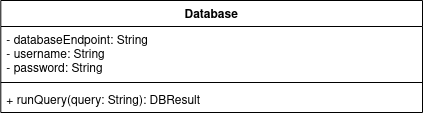
\includegraphics[width=0.9\textwidth]{diagrams/class-database.png}
    \end{figure}

    La classe dedita a comunicare col database, mandandogli le query e ritornando il risultato ricevuto.

    \begin{figure}[htp]
        \centering
        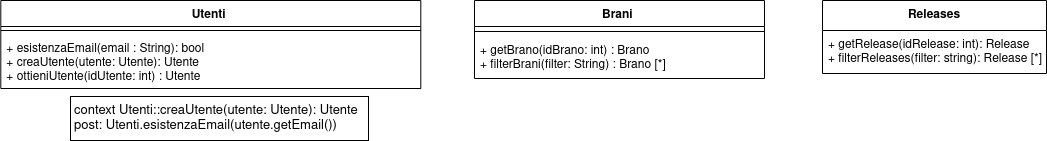
\includegraphics[width=0.9\textwidth]{diagrams/class-odm.png}
    \end{figure}

    \item \label{utenti} \textbf{Utenti}

    La classe Utenti implementa un'interfaccia utile per la gestione degli utenti nel database. L'OCL specifica che, dopo la chiamata a \texttt{creaUtente}, la mail usata nella creazione deve essere nel database, indipendentemente dal fatto che l'utente sia stato inserito o che l'indirizzo mail fosse già presente.

    \item \label{brani} \textbf{Brani}

    La classe Brani implementa un'interfaccia utile per la gestione dei singoli brani nel database. Oltre ad ottenere un brano dal suo ID, è possibile ottenere una lista di brani filtrando quelli nel database.

    \item \label{releases} \textbf{Releases}

    La classe Releases implementa un'interfaccia utile per la gestione delle Releases (Albums, Singoli, EPs, etc...) nel database. Anche qui è possibile ottenere una Release attraverso il suo ID e filtrare tra tutte quelle disponibili.

    \newpage

    \begin{figure}[htp]
        \centering
        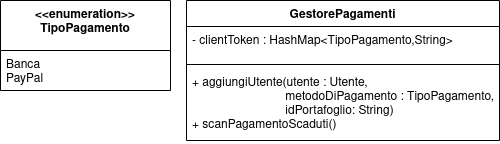
\includegraphics[width=0.9\textwidth]{diagrams/class-payments.png}
    \end{figure}

    \item \label{payments} \textbf{GestorePagamenti}

    La classe è un singleton dedito all'aggiungere abbonamenti al database. \\
    \texttt{aggiungiUtente} viene chiamato alla fine del flow di autorizzazione gestito dal metodo di pagamento stesso (es. Autenticazione e Autorizzazione attraverso l'endpoint OAuth di PayPal), dove \texttt{idPortafoglio} è un token dato dalla piattaforma per il pagamento utile per richiedere il pagamento ogni volta che l'abbonamento scade per il rinnovo automatico. \\
    Una volta ogni giorno viene lanciato \texttt{scanPagamentoScaduti}, che scorre il database per provare a rinnovare gli abbonamenti scaduti. \\
    \texttt{clientToken} è una HashMap che mappa le piattaforme ai presunti \texttt{clientId} richiesti per identificare l'applicazione, ad esempio in uno dei flow di autorizzazione OAuth. \\
    \texttt{TipoPagamento} è l'enumerazione che elenca le piattaforme di pagamento supportate.

    \newpage

    \begin{figure}[htp]
        \centering
        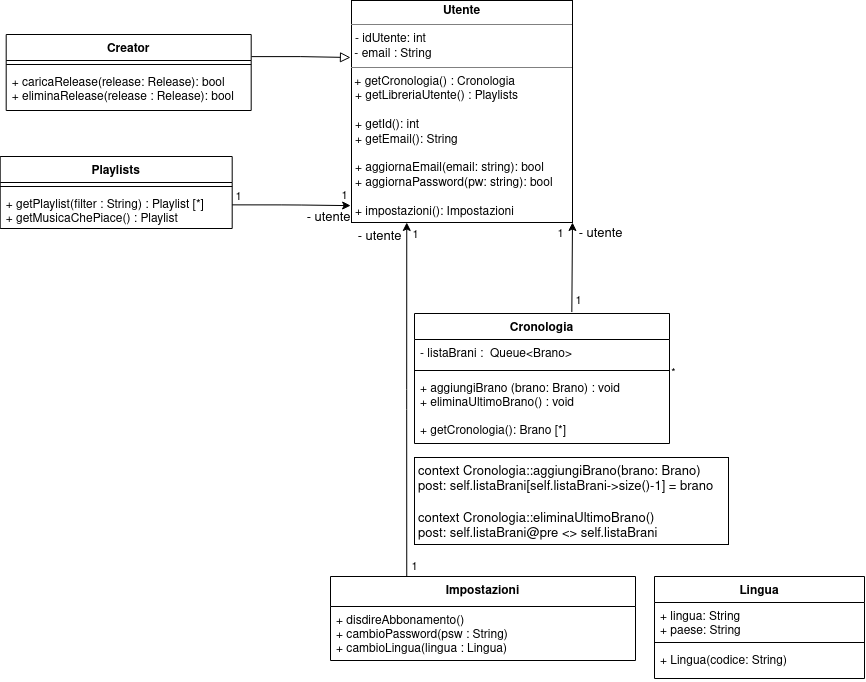
\includegraphics[width=0.9\textwidth]{diagrams/class-user.png}
    \end{figure}

    \item \label{utente} \textbf{Utente e Creator}

    Le classi rappresentano gli oggetti nel database, le funzioni \texttt{aggiornaEmail} e \texttt{aggiornaPassword} modificano anche l'oggetto nel database, ma possono fallire (ad esempio se l'indirizzo mail non è unico o se la password non risponde alle policy).\\
    Alcuni dei metodi ritornano altre classi utili per fare query al database unicamente riguardo un utente.\\
    Il Creator, per l'applicazione, differisce solo nelle operazioni che può fare, dedite alla gestione delle sue Releases.

    \item \label{proxies} \textbf{Playlists, Cronologia e Impostazioni}

    Queste classi possono essere create solo da oggetti Utente e sono utili per fare queries al database filtrando automaticamente per utente.\\
    \texttt{Impostazioni} ha metodi per cambiare alcune preferenze dell'utente.\\
    \texttt{Playlists} permette di ottenere le playlist create dall'utente e la sua playlist 'Musica Che Mi Piace'. \texttt{Playlists} fa le query in maniera 'pigra', ovvero le queries sono mandate solo quando necessario invece di domandare direttamente tutte le playlists al database.\\
    \texttt{Cronologia} permette di ottenere la recente cronologia dell'utente. L'OCL specifica che, una volta chiamato \texttt{aggiungiBrano}, il brano passato come parametro deve risultare come l'ultimo aggiunto, e che \texttt{eliminaUltimoBrano} porti a una lista diversa.\\

    \item \label{lingua} \textbf{Lingua}

    \texttt{Lingua} è una classe utile per confermare che la stringa passata al costruttore sia valido ISO 639.

    \newpage

    \begin{figure}[htp]
        \centering
        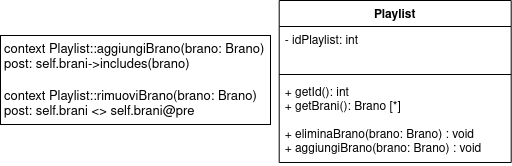
\includegraphics[width=0.9\textwidth]{diagrams/class-playlist.png}
    \end{figure}

    \item \label{playlist} \textbf{Playlist}

    \texttt{Playlist} è l'oggetto che rappresenta una playlist. L'attributo \texttt{brani} è dato dalla relazione con \texttt{Brani}.\\
    L'OCL specifica che, una volta aggiunto un brano, questo dev'essere presente nella playlist, e che una volta rimosso un elemento, la lista dev'essere diversa.

    \begin{figure}[htp]
        \centering
        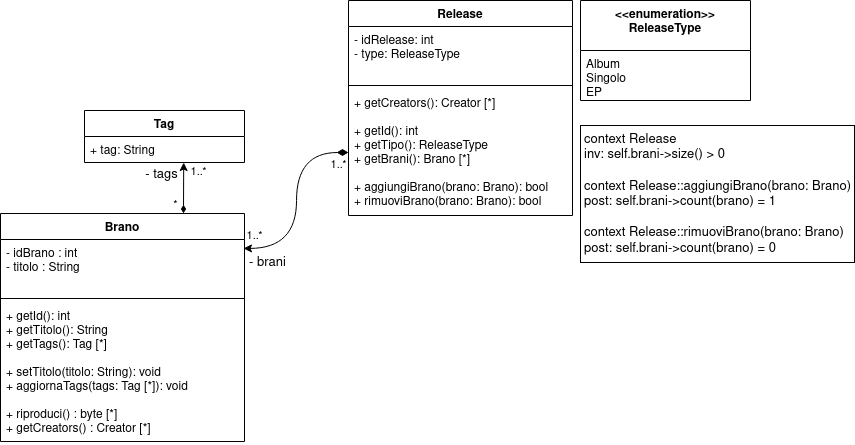
\includegraphics[width=0.9\textwidth]{diagrams/class-media.png}
    \end{figure}

    \item \label{release} \textbf{Release}

    Questo oggetto rappresenta una Release, l'OCL specifica che la lista di brani non dev'essere mai vuota e che ogni brano può apparire una sola volta.\\
    \texttt{getCreators} permette di ottenere la lista di Creators proprietari della Release.
    \texttt{ReleaseType} è un'enumerazione che lista i tipi di Release.

    \item \label{brano} \textbf{Brano}

    \texttt{Brano} rappresenta un Brano nel database, \texttt{getTags} permette di ottenere tutti i suoi tags, \texttt{getCreators} permette di ottenere tutti i suoi Creators, e \texttt{riproduci} ritorna l'array di bytes che compone il file.

    \newpage

    \begin{figure}[htp]
        \centering
        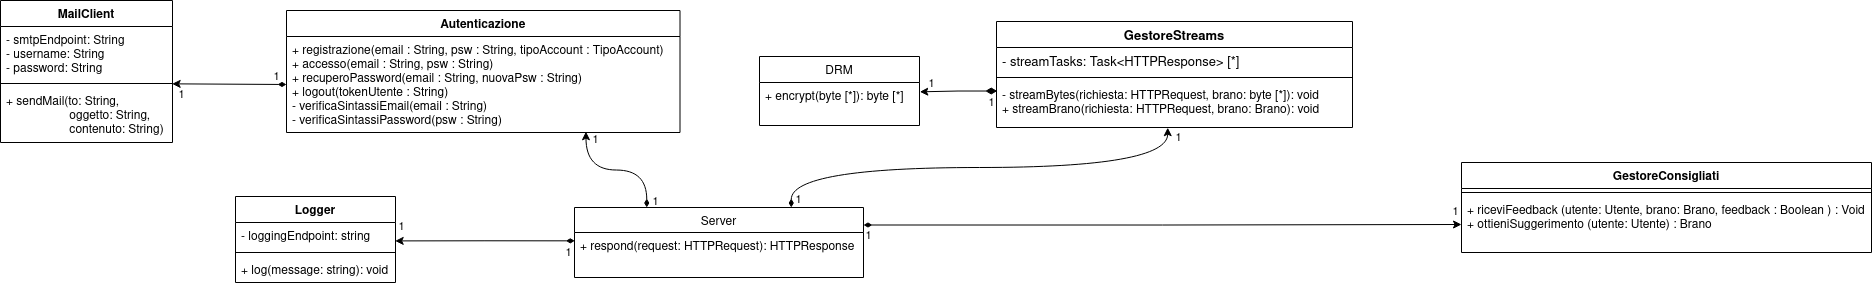
\includegraphics[width=0.9\textwidth]{diagrams/class-server.png}
    \end{figure}

    \item \label{server} \textbf{Server}

    Questo oggetto si premura di rispondere alle richieste HTTP che arrivano al server, smistandole in base a directory richiesta e il loro contenuto.

    \item \label{logger} \textbf{Logger}

    \texttt{Logger} manda i messaggi di log al server adibito a raccoglierli.

    \item \label{consigliati} \textbf{GestoreConsigliati}

    Su richiesta del client GestoreConsigliati ritorna una canzone da consigliare all'utente e registra i feedback dati ai vari suggerimenti.

    \item \label{streams} \textbf{GestoreStreams e DRM}

    Ogni volta che una canzone è richiesta, \texttt{GestoreStreams} lancia un Task per streammare asincronamente al client il file. Il file passa prima per il DRM in modo da venire cifrato in trasporto.

    \item \label{auth} \textbf{Autenticazione e MailClient}

    Autenticazione si premura di gestire registrazione, login, logout e recupero password, e manda mails attraverso il MailClient in caso di registrazione o recupero.

    \newpage

    \begin{figure}[htp]
        \centering
        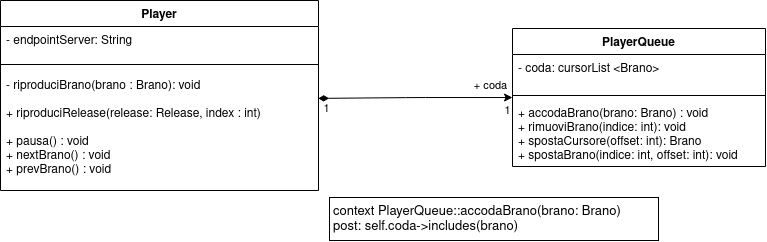
\includegraphics[width=0.9\textwidth]{diagrams/class-client.png}
    \end{figure}

    \item \label{player} \textbf{Player}

    Il Player è nel client e manda le richieste al server per ottenere informazioni e streammare audio.

    \item \label{queue} \textbf{PlayerQueue}

    La Coda del client gli permette di tracciare le tracce richieste e di navigare tra quelle già riprodotte e da riprodurre
\end{enumerate}

\newpage
\section{Diagramma delle classi con OCL}

\begin{figure}[htp]
    \centering
    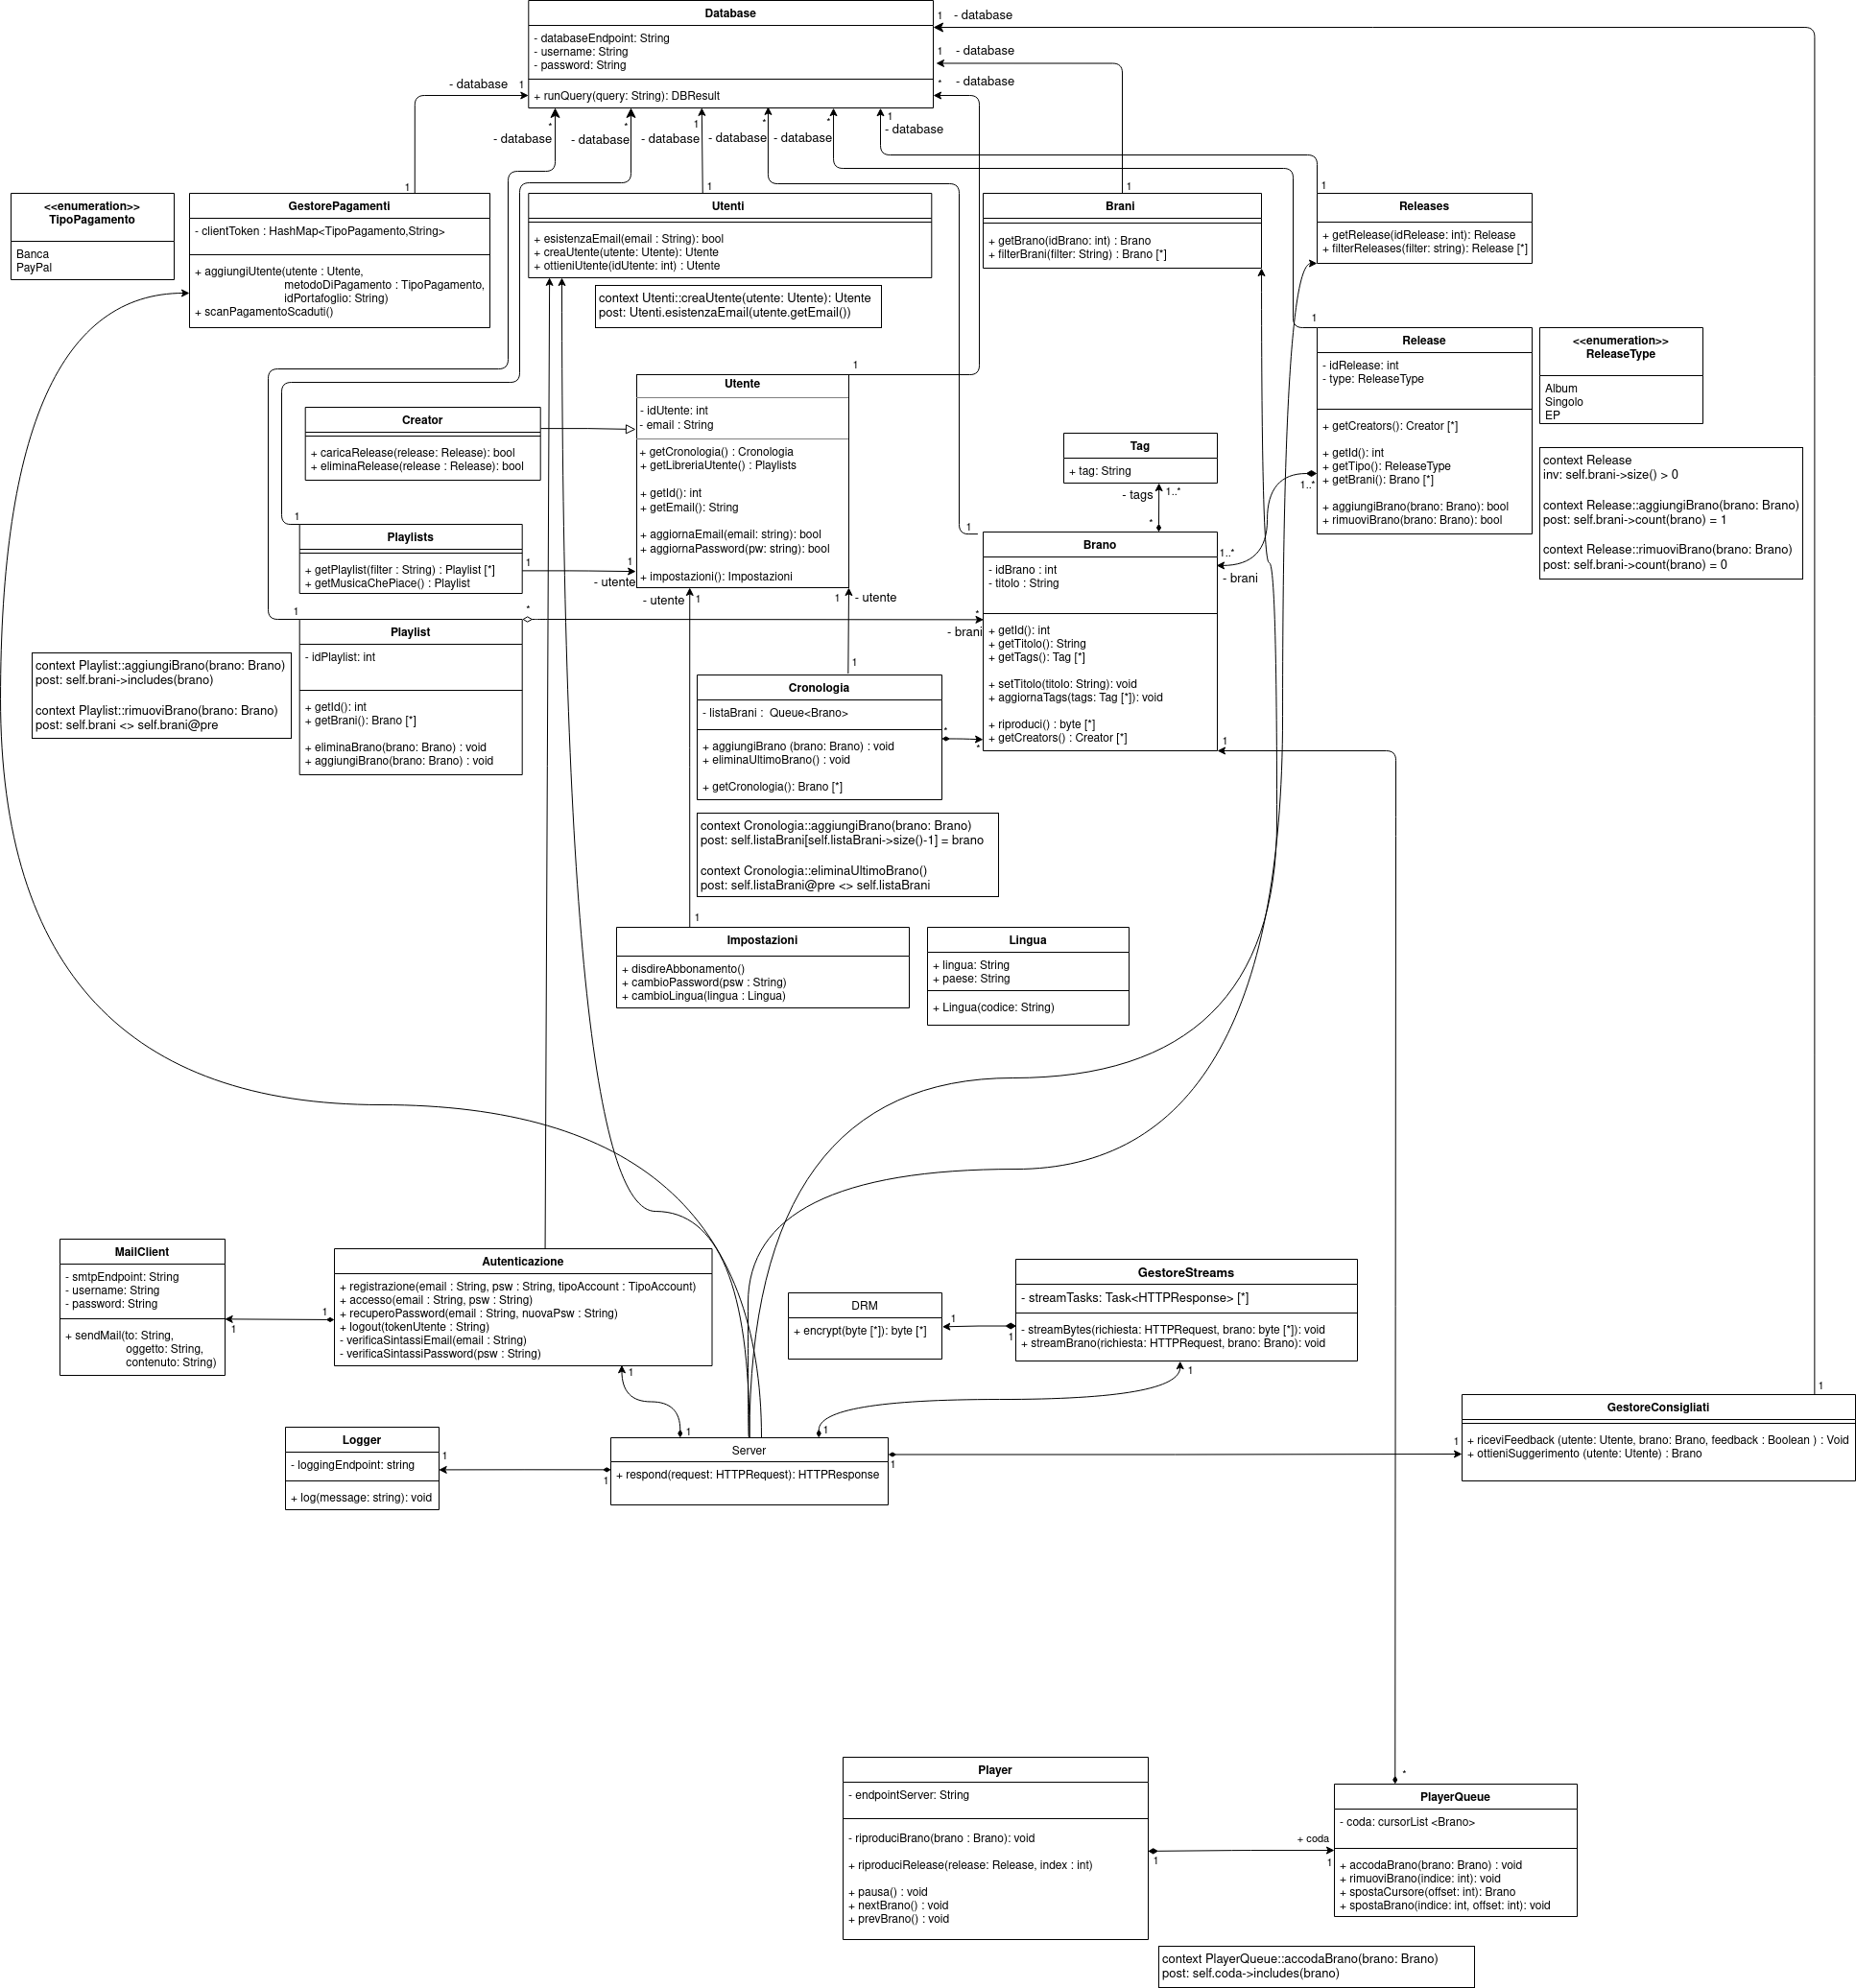
\includegraphics[width=0.9\textwidth]{diagrams/class.png}
\end{figure}

\end{document}